\section{METHOD}

Our pipeline turns a monocular video of human motion into a policy that can be tested and run on a humanoid robot. The user provides the video and selects a robot supported by GMR~\cite{gmr}. The pipeline handles 3D motion generation, retargeting, motion correction, policy training, and deployment. An overview of the stages is shown in Fig.~\ref{fig:pipeline_strip}.

\begin{figure}[t]
    \centering
    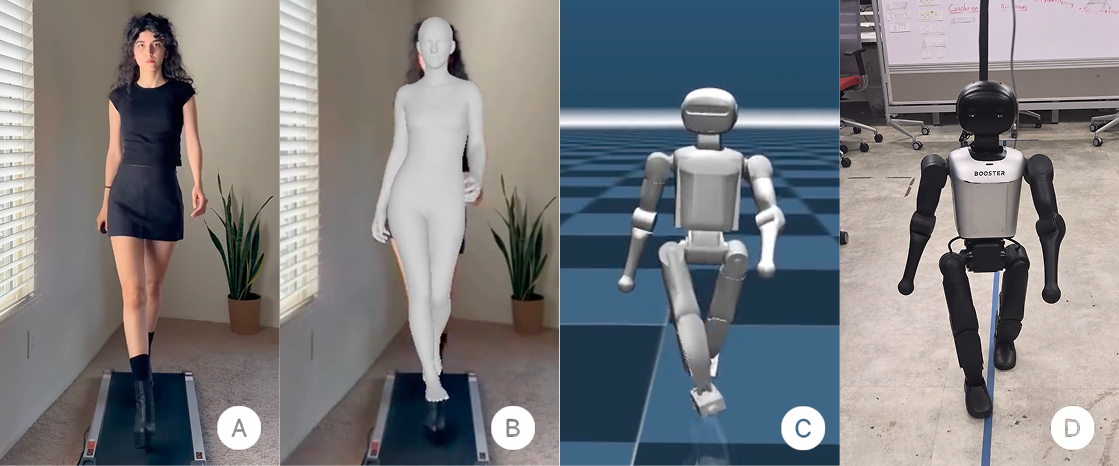
\includegraphics[width=\columnwidth]{figures/pipeline_strip.png}
    \caption{Overview of the pipeline: (a) monocular runway video, (b) recovered 3D human motion, (c) retargeted robot motion in simulation, and (d) physical deployment on the Booster K1.}
    \label{fig:pipeline_strip}
\end{figure}

\subsection{Motion Recovery}

The pipeline uses GVHMR~\cite{gvhmr} to convert the input video into 3D human motion. It reads the video's frame rate and selects the setting for a static or moving camera. The resulting SMPL-X motion and global path are then sent to the retargeting stage.

\subsection{Robot Retargeting}

The user selects a robot supported by GMR~\cite{gmr}. GMR adapts the human motion to the robot's body proportions and joints. The output is a motion trajectory for that robot.

\subsection{Motion Correction and Conversion}

After retargeting, the pipeline detects foot contacts and adjusts the motion to keep the feet aligned with the floor. It also removes vertical drift without changing the joint angles, preserving the original walking style. Finally, the motion is converted into the training format with the robot joint states, base pose, and frame timing from the source video.

\subsection{Policy Training}

The processed motion is used as the reference trajectory for training with BeyondMimic~\cite{beyondmimic} in the Booster training framework~\cite{boostertrain}. We use the existing training method while keeping the actuator limits, stiffness, damping, and action scaling consistent with the deployment configuration. This avoids using a policy on hardware with different control settings from those used during training.

\subsection{Simulation and Deployment}

After training, the exported policy is loaded into the Booster deployment framework~\cite{boosterdeploy} and tested in MuJoCo using the deployment controller. This sim-to-sim test is used to check balance, tracking, and joint behavior before hardware execution. The same exported policy can then be launched on the physical robot with our deployment script. The final output of the workflow is therefore a runnable robot policy rather than only a retargeted trajectory or training checkpoint.
